\begin{figure}[ht]
\centering
\newcommand\dapgwidth{0.16}
\subfloat[\texttt{Hammer} environment. ]{
\begin{tabular}{c}
\addvbuffer[0pt 0pt]{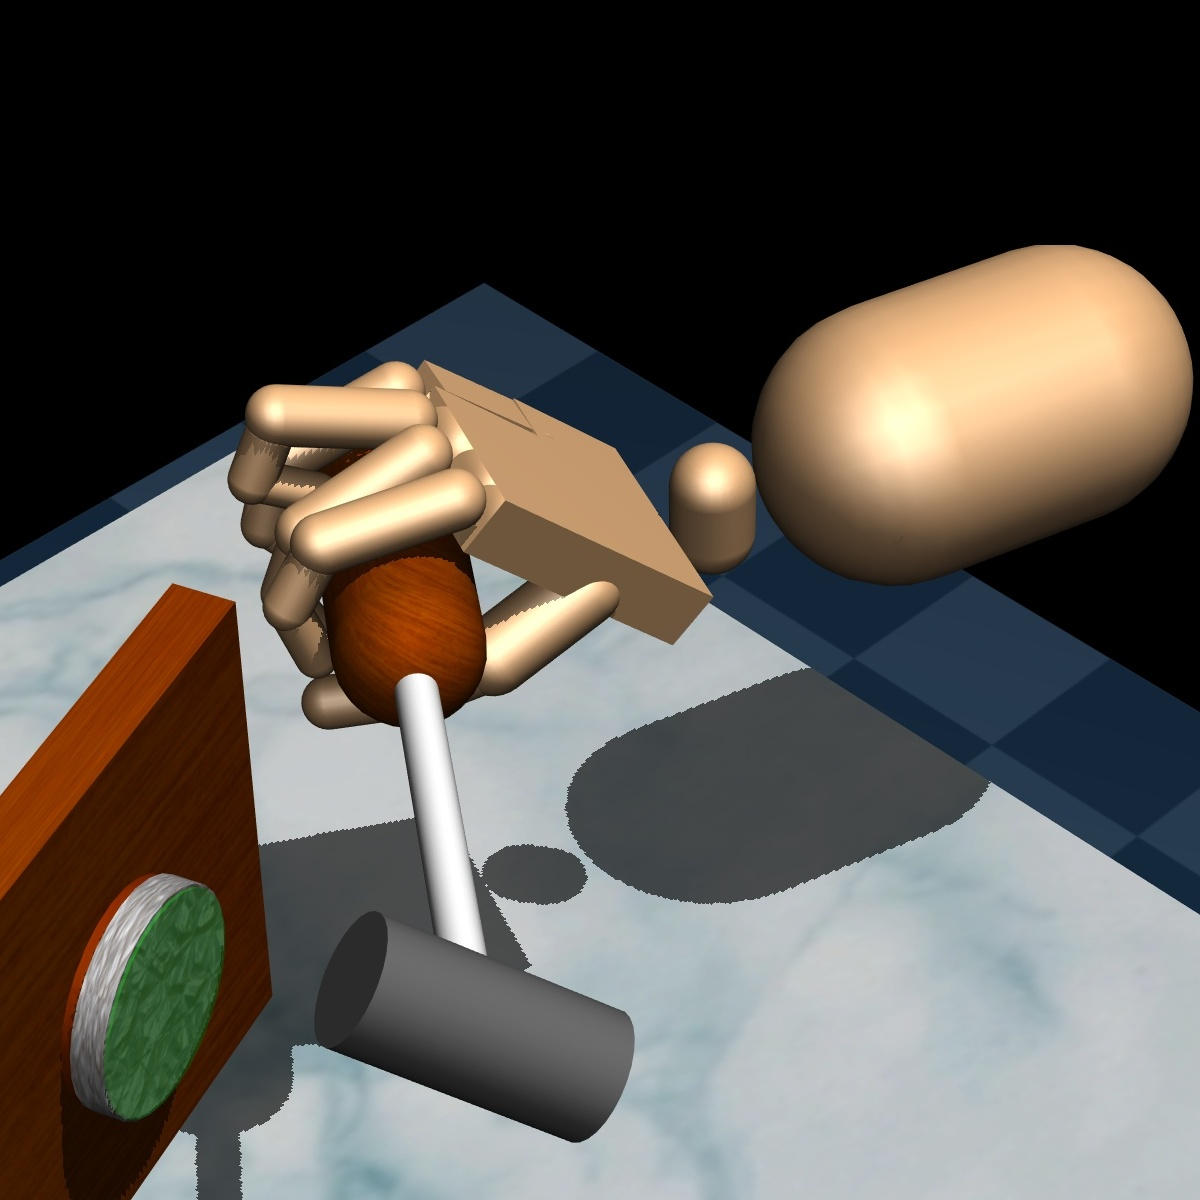
\includegraphics[width=\dapgwidth\textwidth, valign=m]{Figures/dapg/hammer_0.jpg}} $\rightarrow$ \addvbuffer[0pt 0pt]{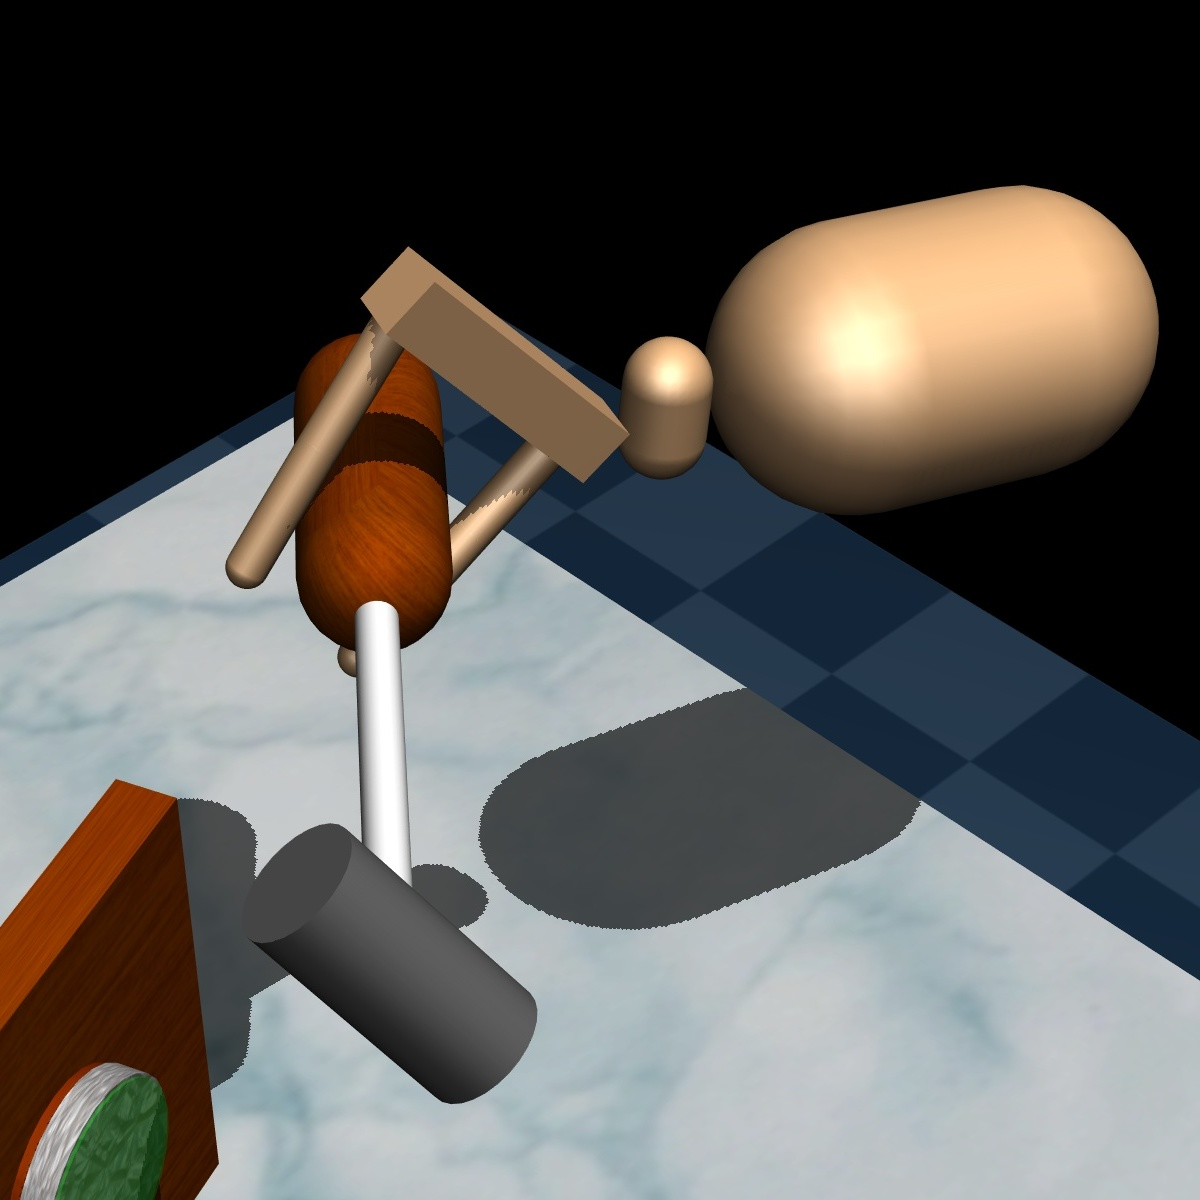
\includegraphics[width=\dapgwidth\textwidth,valign=m]{Figures/dapg/hammer_1.jpg}}
\end{tabular} 
} 
\vspace{-2ex}
\\
\subfloat[\texttt{Relocate} environment. ]{
\begin{tabular}{c}
\addvbuffer[0pt 0pt]{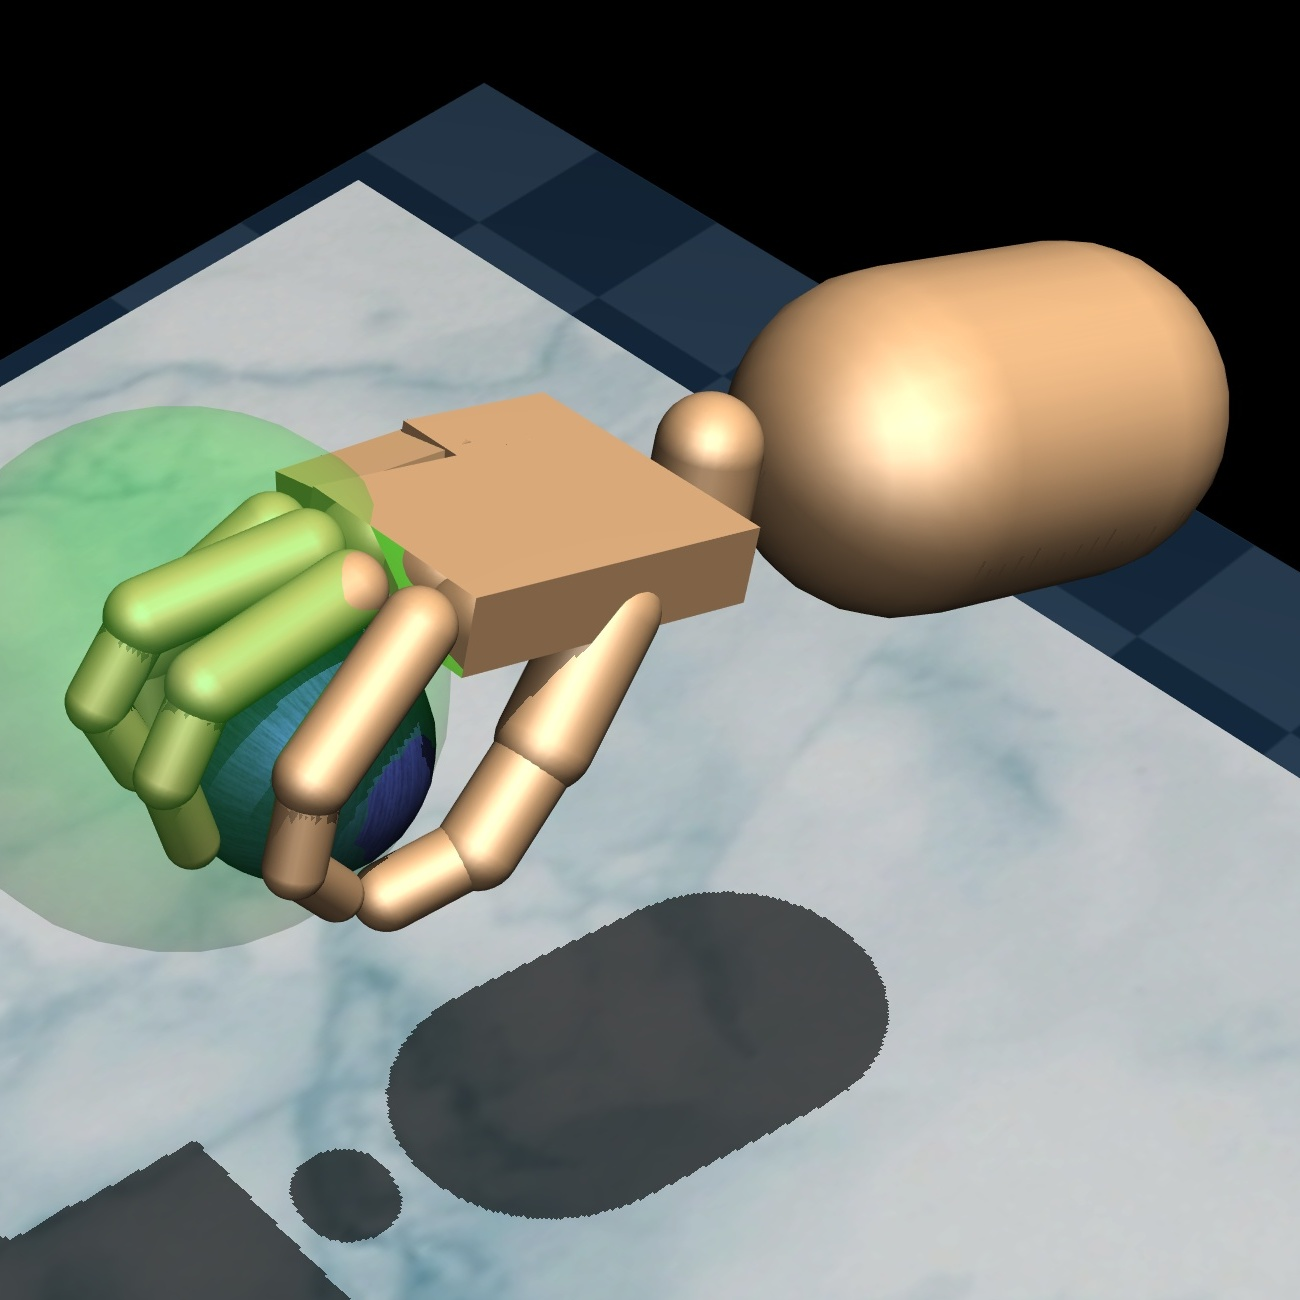
\includegraphics[width=\dapgwidth\textwidth, valign=m]{Figures/dapg/relocate_0.jpg}} $\rightarrow$ \addvbuffer[3pt 0pt]{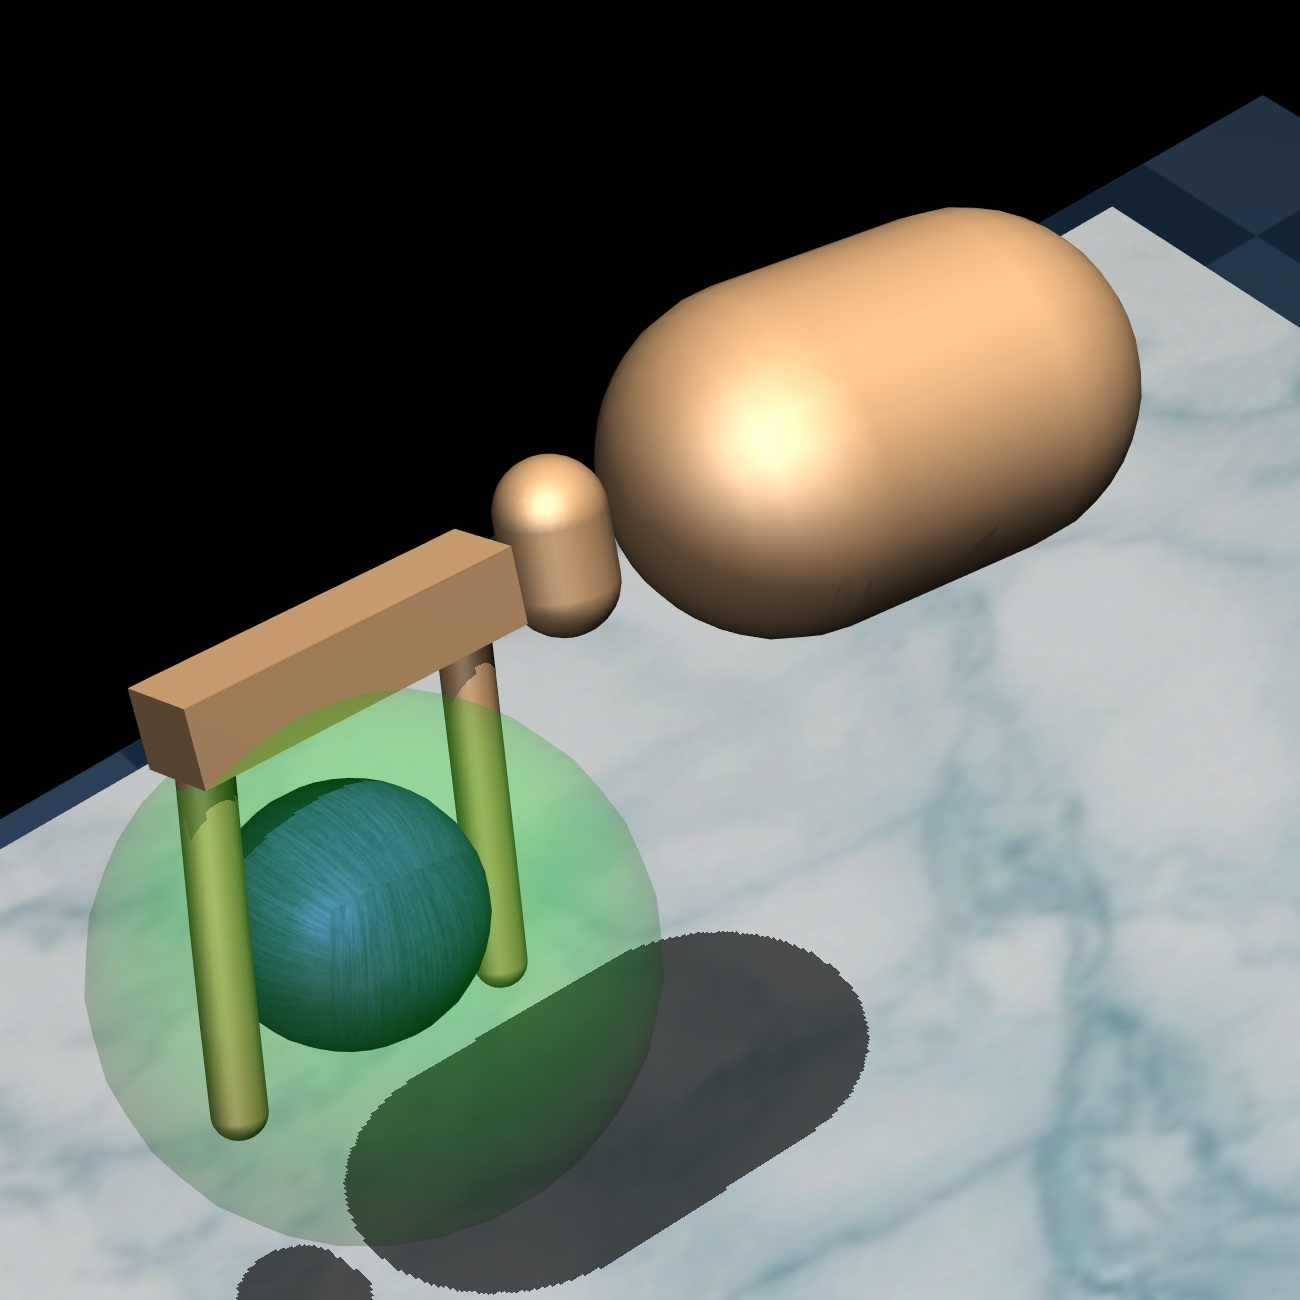
\includegraphics[width=\dapgwidth\textwidth,valign=m]{Figures/dapg/relocate_1.jpg}} 
\end{tabular} 
} 
\vspace{-2ex}
\\
\subfloat[\texttt{Door} environment. ]{
\begin{tabular}{c}
\addvbuffer[0pt 0pt]{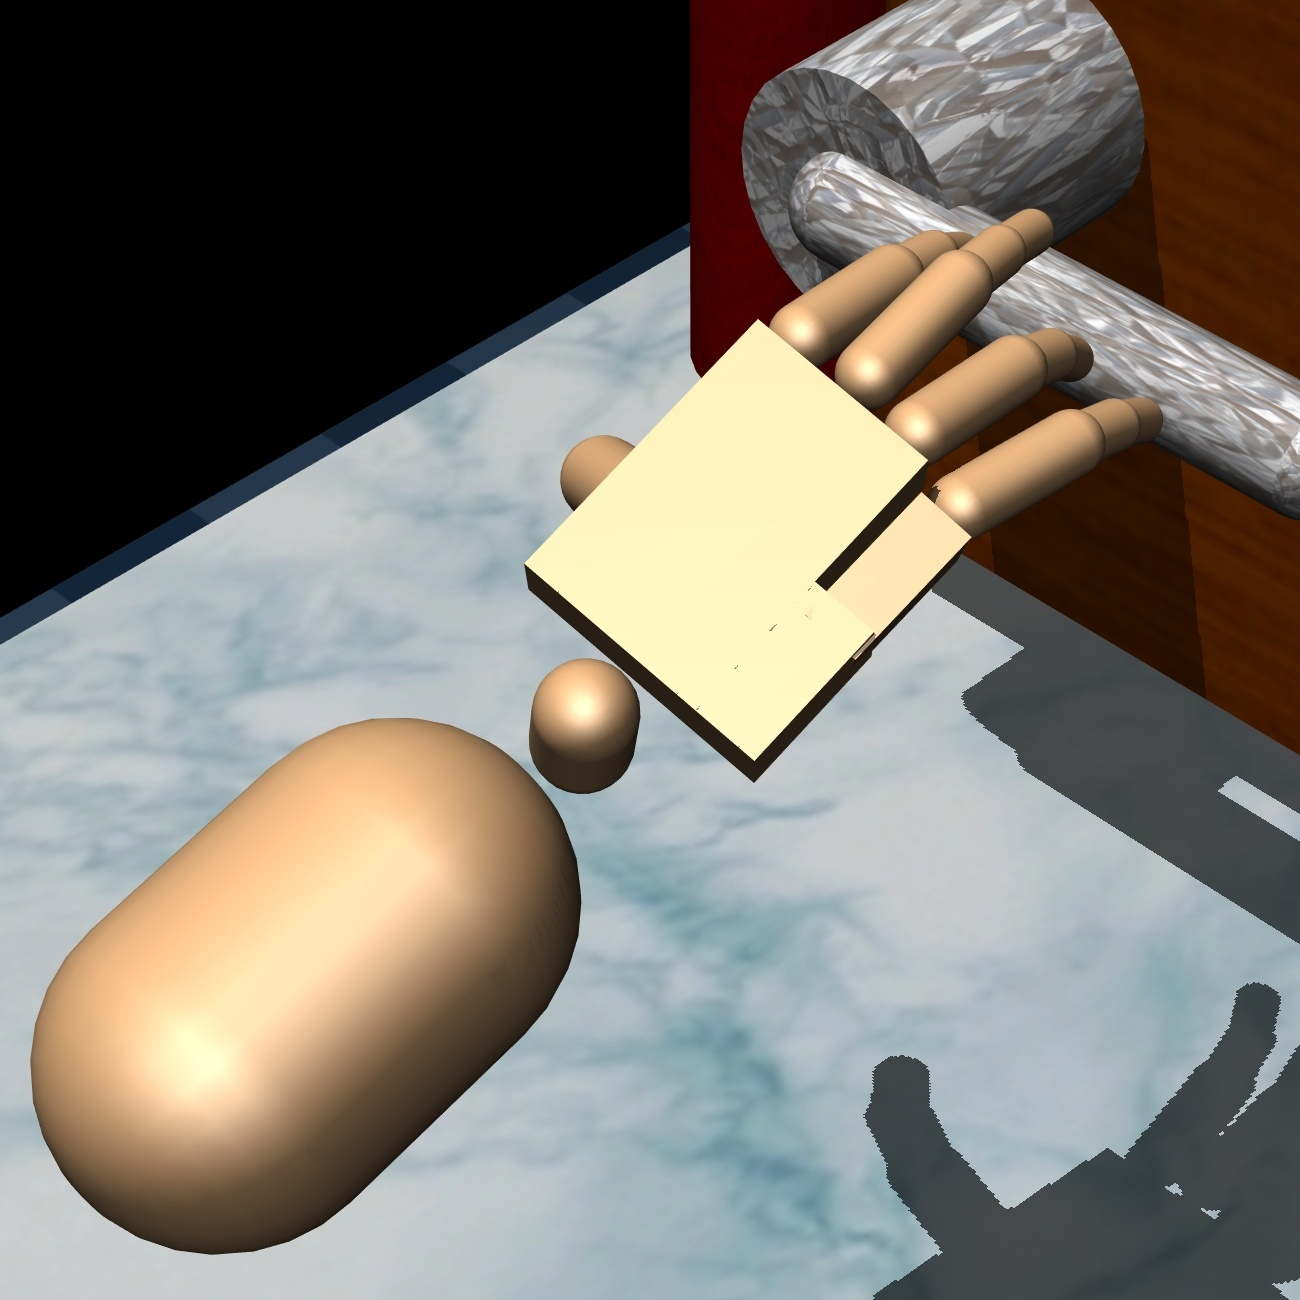
\includegraphics[width=\dapgwidth\textwidth, valign=m]{Figures/dapg/door_0.jpg}} $\rightarrow$ \addvbuffer[3pt 0pt]{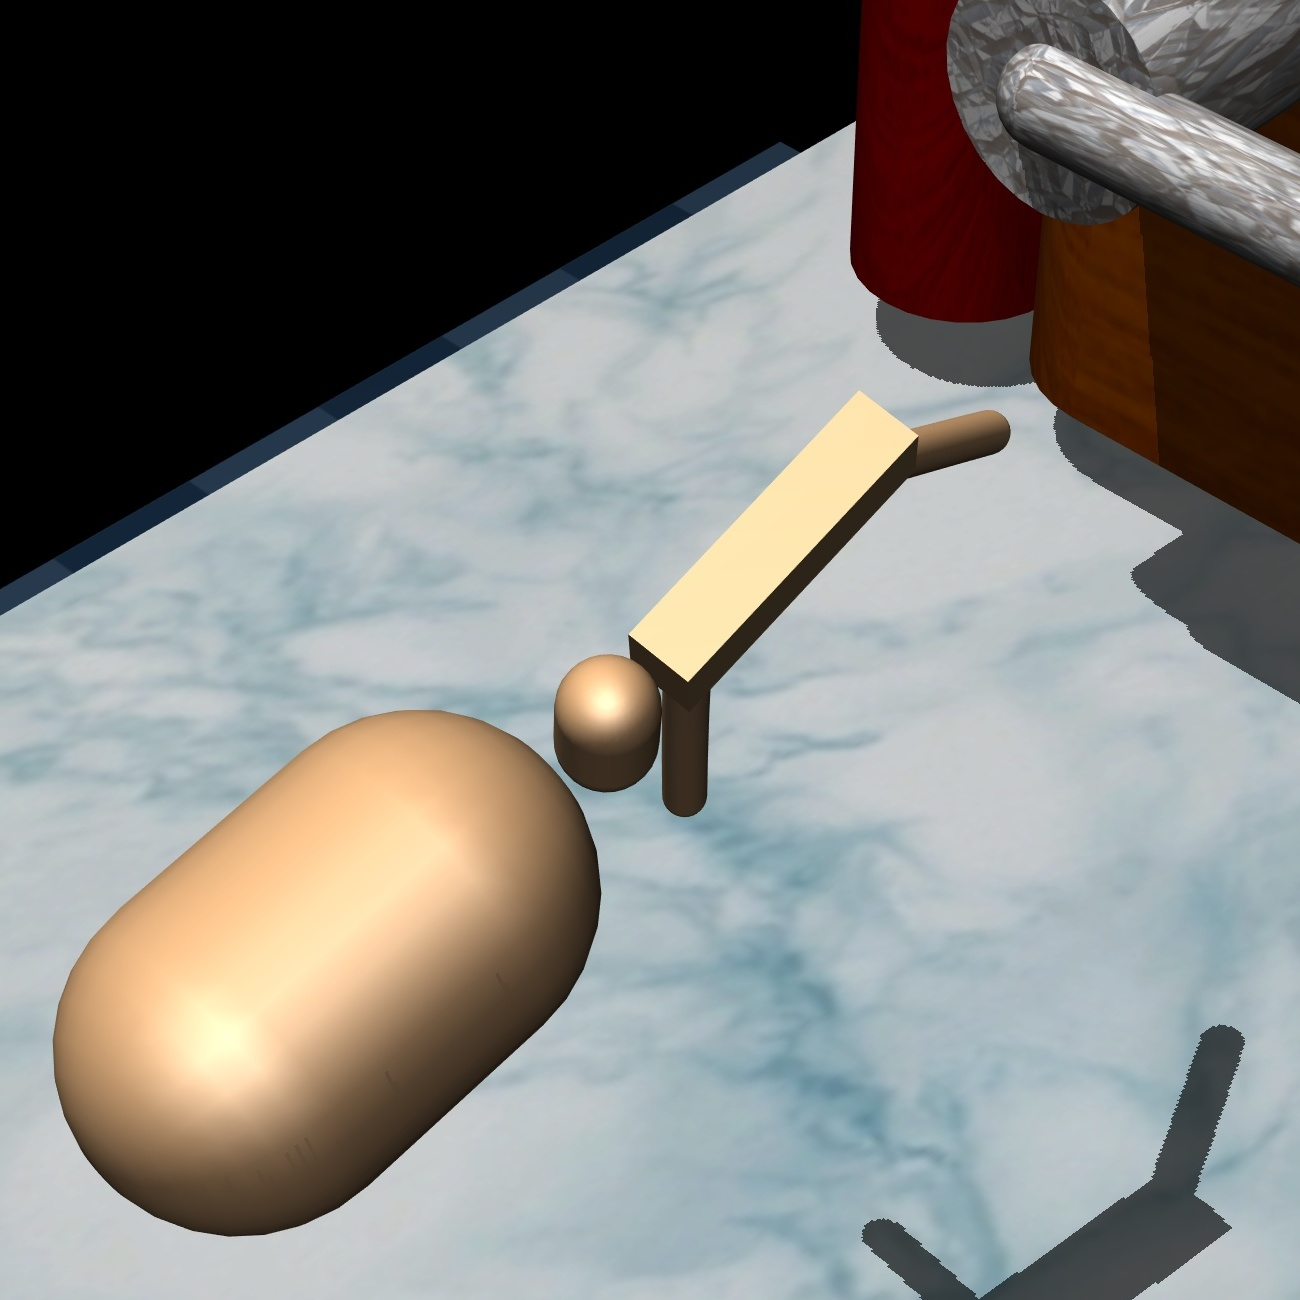
\includegraphics[width=\dapgwidth\textwidth,valign=m]{Figures/dapg/door_1.jpg}} \\
\end{tabular}
} 
\vspace{-1ex}
\caption{\textbf{Hand Manipulation Suite tasks.}
(a) \texttt{Hammer} environment. The goal is to pick up the hammer and smash the nail into the board;
(b) \texttt{Relocate} environment. The goal is to pick up the blue ball and take it to the desired site denoted as green sphere;
(c) \texttt{Door} environment. The goal is to switch the latch and fully open the door.
}
\label{fig:dapg}
\end{figure}

